\documentclass{article}
\usepackage{amsmath}
\usepackage[margin=1in]{geometry}
\usepackage{amsfonts}
\usepackage{hyperref}
\usepackage{graphicx}
\usepackage{longdivision}

\begin{document}
	
	\title{Computer Numerical Representation}
	\author{Andy Chong Sam}
	\maketitle
	
	\section{Introduction} 
	\par\noindent Math is most commonly performed using a decimal system. We call this a decimal system because ten symbols are used: \(\{0,1,2,3,4,5,6,7,8,9\}\). Any number can be decomposed using a member from the set of symbols and a power of ten, take the number \(1421\) for example, which can be written as:
	
	\begin{flalign*}
		1421 = (1)(10)^3 + (4)(10)^2 + (2)(10)^1 + (1)(10)^0
	\end{flalign*}

	\par\noindent Computers use a binary system, where the set of usable symbols has been reduced to just two: \(\{0,1\}\). This is referred to as a binary system. This document explains the algorithms to convert between decimal and binary systems. It will also explain how negative and fractional amounts are represented in binary.
	
	\section{Decimal to Binary}
	\par\noindent The algorithm to translate decimal to binary involves repeated divisions by 2, and recording the remainders. The stopping point is when the dividend becomes 1. The list of remainders is then reversed. We will use the same number as before, 1421 to illustrate this.
	
	\begin{flalign*}
		\intlongdivision{1421}{2} \intlongdivision{710}{2} \intlongdivision{355}{2}\intlongdivision{177}{2}
		\intlongdivision{88}{2} \intlongdivision{44}{2} \intlongdivision{22}{2} \intlongdivision{11}{2} 
		\intlongdivision{5}{2} \intlongdivision{2}{2} \intlongdivision{1}{2}
	\end{flalign*}

	\par\noindent The recorded list of remainders is \(10110001101\). Reversing the list gets us the binary representation of 1421: \(10110001101\). 
	
	\section{Binary to Decimal}
	
	\par\noindent Let's try the reverse process now. Suppose that I have \(10110001101\) and I want to transform that into a decimal number. Similar to the example in the introduction, we can assign place
	values to all the binary digits:
	
	\begin{center}
		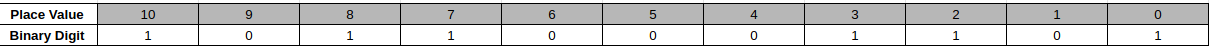
\includegraphics[width=18cm]{place.png}
	\end{center}

	\par\noindent We then proceed to multiply each binary digit by two raised to the place value. All these terms will then be added together:

 	\begin{flalign*}
 		2^{10} + 2^8 + 2^7 + 2^3 + 2^2 + 1 = 1421
 	\end{flalign*}

	\section{Negative Integers}
	
	\par\noindent The binary equivalent of a negative number is formulated using the two's complement technique. First, we take the one's complement which involves flipping each zero to a one, and each one to a zero. Finally we add a binary 1. Suppose we wanted to represent -1421:
	
	\begin{center}
	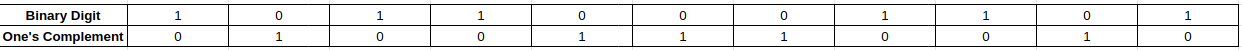
\includegraphics[width=18cm]{two-comp-1.png}
	\end{center}

	\begin{center}
	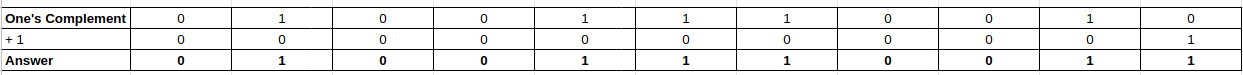
\includegraphics[width=18cm]{two-comp-2.png}
\end{center}
	
	\par \noindent We are left with the result \textbf{01001110011}. This result occupies 10 positions (or 11 bits). In an actual computer, the most significant bit is known as the \textbf{sign bit}, and for negative numbers it will be set to 1. The left most bit is the most significant bit.
	\newline

	\par \noindent If we above result was processed through a 12 bit computer, -1421 would be stored as \textbf{101001110011}.
	
	\par\noindent 


\end{document}